\documentclass[11pt]{article}
\usepackage{amsmath}
\usepackage{geometry}
\geometry{margin=1in}
\usepackage{xcolor}
\usepackage{graphicx}
\pagecolor{white}

% --- Author and Title Information ---
\title{COMPSCI 589: Machine Learning - Homework 1}
\author{Vishnu Vardhan Reddy Bheem Reddy}

\begin{document}

\maketitle

% ================================
\section*{Question 1: KNN and Data Scaling}

\noindent
My immediate answer is no, the KNN classification function is not invariant when different scale factors are used for different dimensions.

\medskip
\noindent
The reason is that this scaling changes the geometry of the feature space. The Euclidean distance between two re-scaled points $x'_i$ and $x'_j$ becomes a weighted distance:
\[
d(x'_i, x'_j) = \sqrt{\sum_{d=1}^{D} \left(\frac{x_{id}}{s_d} - \frac{x_{jd}}{s_d}\right)^2} = \sqrt{\sum_{d=1}^{D} \frac{1}{s_d^2}(x_{id} - x_{jd})^2}
\]
Since each dimension $d$ is weighted differently by $1/s_d^2$, the relative distances between points can change. A point that was the 3rd nearest neighbor in the original space might become the 10th nearest in the scaled space. Because the set of K-nearest neighbors can change, the final classification from the majority vote can also change.

\medskip
\noindent
However, as a side thought, if all dimensions were scaled by the \emph{same} factor, so $s_d = s$ for all $d$, then the classification would be invariant.
All distances are just scaled by a constant factor $1/s$. This preserves the distance rankings, meaning the set of K-nearest neighbors for any point will be identical, and the classification will not change.

% ================================
\section*{Question 2: KNN and Missing Data}

\noindent
My idea is to modify the standard KNN distance calculation to handle the missing values. We can use the binary mask vector, $m_i$, to make sure we only compare the features that are actually present.

\medskip
\noindent
When we calculate the distance between a new point $x$ and a training point $x_i$, we should only consider the dimensions where both vectors have a mask value of 1. We can change the Euclidean distance formula like this:

\[
d'(x,x_i) = \sqrt{\sum_{d=1}^{D} m_d \cdot m_{i,d} \cdot (x_d - x_{i,d})^2}
\]

\noindent
In this formula, the term $m_d \cdot m_{i,d}$ will be 1 only if the feature is present in both vectors. Otherwise, it is 0, so that dimension is ignored in the distance calculation.

\medskip
\noindent
After calculating this new distance for all training points, the rest of the KNN algorithm is the same. We find the $K$ points with the smallest distance and use a majority vote to decide the class.

\medskip
\noindent
My observation is that this might not work well if there are too many missing values, because then we would be comparing points based on very few features. Another thought is to maybe fill the missing values with the mean of the feature, but that might add some bias to the data.

% ================================
\section*{Question 3: Probabilistic KNN}

\noindent
My approach is to prove that the function satisfies the two required conditions for a valid probability mass function (PMF): 1) all probabilities are non-negative, and 2) the probabilities sum to one over all possible outcomes.

\medskip
\noindent
\textbf{1. Non-negativity:}
\noindent
We need to show $P_{KNN}(Y=y|X=x) \geq 0$.
\begin{itemize}
    \item The denominator $\epsilon C + K$ is positive, since the number of classes $C \geq 1$ and the number of neighbors $K \geq 1$.
    \item The indicator function $I(y_i=y)$ is either 0 or 1, so its sum $\sum_{i \in N_K(x)} I(y_i=y)$ is non-negative.
    \item The numerator $\epsilon + (\text{a non-negative sum})$ must therefore be positive.
\end{itemize}
Since we are dividing a positive number by another positive number, the result is always positive. The non-negativity condition holds.

\medskip
\noindent
\textbf{2. Sum to one:}
\noindent
We need to show that $\sum_{y \in \mathcal{C}} P_{KNN}(Y=y|X=x) = 1$.
\[
\sum_{y \in \mathcal{C}} P_{KNN}(Y=y|X=x) = \sum_{y \in \mathcal{C}} \frac{1}{\epsilon C + K} \left(\epsilon + \sum_{i \in N_K(x)} I(y_i = y) \right)
\]
We pull out the constant term and split the summation.
\[
= \frac{1}{\epsilon C + K} \left[ \sum_{y \in \mathcal{C}} \epsilon + \sum_{y \in \mathcal{C}} \left( \sum_{i \in N_K(x)} I(y_i = y) \right) \right]
\]
Evaluating each part of the sum inside the brackets.
\begin{itemize}
    \item The first term is simple: $\sum_{y \in \mathcal{C}} \epsilon = \epsilon C$.
    \item For the second term, we can swap the order of summation:
    \[
    \sum_{i \in N_K(x)} \sum_{y \in \mathcal{C}} I(y_i = y)
    \]
    The inner sum $\sum_{y \in \mathcal{C}} I(y_i = y)$ must equal 1, because for any given neighbor $i$, its label $y_i$ belongs to exactly one class in $\mathcal{C}$. Hence, the second term simplifies to $\sum_{i \in N_K(x)} 1 = K$.
\end{itemize}
Substituting these results back into the equation:
\[
= \frac{1}{\epsilon C + K} \left[ \epsilon C + K \right] = 1
\]
Both conditions are satisfied, so the function is a valid PMF.

% ================================
\section*{Question 4: LDA Probabilistic Prediction}

\noindent
The main idea is to start with Bayes' theorem and substitute the specific definitions for the LDA prior and likelihood.

\medskip
\noindent
First, the foundation for this is Bayes' theorem:
\[
P(Y=y|\mathbf{X}=\mathbf{x}) = \frac{P(\mathbf{X}=\mathbf{x}|Y=y)P(Y=y)}{P(\mathbf{X}=\mathbf{x})}
\]
Next, I'll build the numerator, $P(\mathbf{X}=\mathbf{x}|Y=y)P(Y=y)$, by combining the prior $P(Y=y) = \pi_y$ and the Gaussian likelihood:
\[
P(\mathbf{X}=\mathbf{x}|Y=y) = \frac{1}{|2\pi\Sigma|^{1/2}} \exp\left(-\frac{1}{2}(\mathbf{x}-\mu_y)^T \Sigma^{-1}(\mathbf{x}-\mu_y)\right)
\]
Then, the denominator, $P(\mathbf{X}=\mathbf{x})$, is found by summing the joint probability over all classes $k=1, \dots, C$.
\[
P(\mathbf{X}=\mathbf{x}) = \sum_{k=1}^{C} \pi_k \frac{1}{|2\pi\Sigma|^{1/2}} \exp\left(-\frac{1}{2}(\mathbf{x}-\mu_k)^T \Sigma^{-1}(\mathbf{x}-\mu_k)\right)
\]
Putting it all together, the constant term $\frac{1}{|2\pi\Sigma|^{1/2}}$ appears in the numerator and every term of the denominator, so it cancels out. This leaves the final formula:
\[
P(Y=y|\mathbf{X}=\mathbf{x}) = \frac{\pi_y \exp\left(-\frac{1}{2}(\mathbf{x}-\mu_y)^T \Sigma^{-1}(\mathbf{x}-\mu_y)\right)}{\sum_{k=1}^{C} \pi_k \exp\left(-\frac{1}{2}(\mathbf{x}-\mu_k)^T \Sigma^{-1}(\mathbf{x}-\mu_k)\right)}
\]

% ================================
\section*{Question 5: Optimization}

\noindent
My plan is to use analytic methods to find the minimizers of $f(x) = x^4 - 2x^2 + 1$. 

\medskip
\noindent
\textbf{1. Find Critical Points}

\noindent
First, I'll compute the first derivative of the function $f(x)$ and set it to zero.
\[
f'(x) = 4x^3 - 4x = 4x(x^2 - 1) = 4x(x-1)(x+1)
\]
Setting $f'(x)=0$ gives three critical points: $x = -1$, $x = 0$, and $x = 1$.

\medskip
\noindent
\textbf{2. Classify Critical Points}

\noindent
Next, I'll use the second derivative test. The second derivative is $f''(x) = 12x^2 - 4$.
\begin{itemize}
    \item At $x = -1$: $f''(-1) = 12(-1)^2 - 4 = 8 > 0$, so this is a local minimum.
    \item At $x = 0$: $f''(0) = 12(0)^2 - 4 = -4 < 0$, so this is a local maximum.
    \item At $x = 1$: $f''(1) = 12(1)^2 - 4 = 8 > 0$, so this is a local minimum.
\end{itemize}

\medskip
\noindent
\textbf{3. Identify Global Minimizers}

\noindent
We have two local minima at $x = -1$ and $x = 1$. The value of the function at these points is:
\[
f(1) = (1)^4 - 2(1)^2 + 1 = 0
\]
\[
f(-1) = (-1)^4 - 2(-1)^2 + 1 = 0
\]
Both local minima have a value of 0. Since $\lim_{x \to \pm\infty} f(x) = \infty$, the function increases without bound away from the critical points. Therefore, the local minima we found must be the global minima. The global minimizers are $x = -1$ and $x = 1$.

% ================================
\section*{Question 6: Heart Disease Classification}

\subsection*{a. Data Set Properties}

\noindent
After running the preprocessing steps in the notebook, I found the following properties for the dataset:
\begin{itemize}
    \item Training data cases: 242
    \item Test data cases: 61
    \item Feature dimensions: 18
\end{itemize}

\subsection*{b. Logistic Regression Performance}

\noindent
After evaluating it on both the training and test sets, I found the following error rates:
\begin{itemize}
    \item Training error rate: 0.1240
    \item Test error rate: 0.1639
\end{itemize}

\subsection*{c. K-Nearest Neighbors Performance}

\noindent
\begin{figure}[h!]
\centering
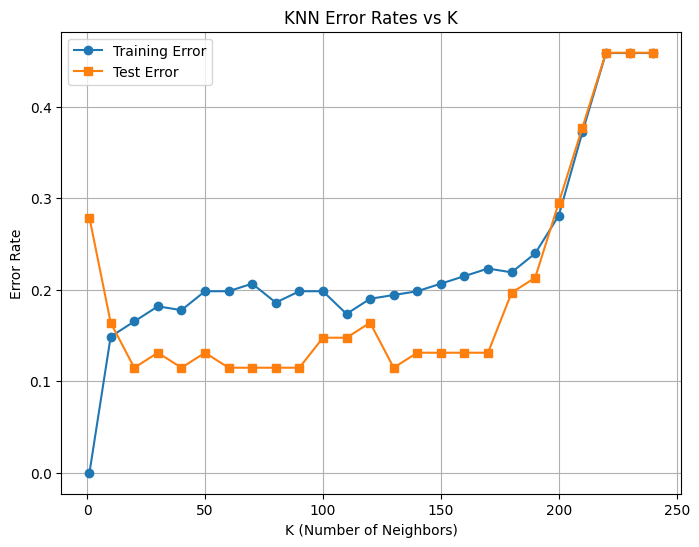
\includegraphics[width=0.8\textwidth]{img.png}
\caption{Training and test error rates for the KNN classifier as a function of the number of neighbors (K).}
\label{fig:knn}
\end{figure}

\subsection*{d. Baseline LLM Performance}

\noindent
I ran the initial `llm.ipynb` notebook on a T4 GPU in Google Colab. This version used the simple starter prompt, which only provides the patient's age to the Falcon-H1-3B-Instruct model.
\begin{itemize}
    \item Test error rate: 0.4587   
\end{itemize}

\subsection*{e. Prompt Engineering with More Features}

\noindent
My next idea was to see if providing more features would improve the LLM's performance. I experimented with two new prompt structures and compared them against the baseline on the training data:
\begin{itemize}
    \item \textbf{Full Narrative:} A descriptive sentence that combines all features into a paragraph (e.g., "Age 52, sex: male, chest pain type: asymptomatic...").
    \item \textbf{Key-Value Concise:} A comma-separated list of feature names and their values (e.g., "age: 52, sex: male, cp: asymptomatic...").
\end{itemize}
The "Full Narrative" prompt performed best on the training data, achieving a training error of 0.3388. After selecting this as my best prompt, I ran it on the test set.
\begin{itemize}
    \item Test error rate (Best Prompt): 0.2131
\end{itemize}

\subsection*{f. Few-Shot Prompting}

\noindent
To give the small model more context, I tried a "few-shot" prompting strategy. My idea was to provide examples within the prompt itself to guide the model's classification. The prompt was structured to show the model three example patients without heart disease and three examples with heart disease, all taken from the training set, before presenting the actual test case for classification.
\begin{itemize}
    \item Test error rate (Few-Shot Prompt): 0.3115
\end{itemize}

\subsection*{g. Generative AI Usage}

\noindent
For Question 6 (parts d, e, and f), I utilized a generative AI assistant to help with the implementation in the `llm.ipynb` notebook. My use of the tool was focused on improving code efficiency and formatting. I prompted the assistant to help structure a batch processing loop to ensure the code would run without memory errors on the GPU. I also used it for minor syntax corrections and for help formatting the multi-line prompt strings.

\end{document}